\chapter{Foundations}
\label{chapter2}

This thesis draws upon prior research from the robotics, information theory, and signal
processing domains to develop its formulations.
Sections~\ref{sec:occ_grid_mapping} - \ref{sec:action_generation} review relevant topics within
robotics including occupancy grid mapping,
active perception as an optimization, and several planning strategies that are suitable for the
exploration task. These foundational topics will be used to develop a theory of
optimal occupancy grid compression as well as methods for guiding a robot to explore
uncertain areas of its map efficiently. The formulations developed in
Chapters~\ref{chapter3} - \ref{chapter5} will also
borrow heavily from information theory and rate distortion theory. These
domains are frequently concerned with evaluating the effect one random
variable (e.g. a sensor measurement) has on
another (e.g. a map) or with compressing a random variable to a reduced
representation in such a way that the compressed form preserves the structure of the
uncompressed form.
Sections~\ref{sec:entropy_and_divergence} and \ref{sec:csqmi} review concepts from
these domains that will be used when developing theories for optimal map resolution selection,
and for adapting robot exploration behaviors to the resolution with which its environment is
modeled.

\section{Occupancy Grid Mapping}
\label{sec:occ_grid_mapping}

Occupancy grids (OGs) are a common and useful proabilistic map model for representing and
reasoning about an unknown environment. The remainder of this
thesis assumes that the robot's environment is represented as an OG.
Figures~\ref{fig:frontiers},~\ref{fig:sensor_frontier} and~\ref{fig:og} depict occupancy grids,
where black cells represent areas of the environment occupied by an obstacle, white cells
represent areas that do not contain obstacles, and grey cells represent
locations with unknown occupancy status.

OGs decompose the robot's workspace into a discrete set of 2D or 3D cells with a
specified resolution. The presence or absence of obstacles within these cells is modeled
as a $K$-tuple binary random variable, $\mbf{m} = \{m_{i}\}_{i=1}^{K}$, with support set
$\{\texttt{EMP}, \texttt{OCC}\}$. The probability that an individual cell is occupied is
given by $p\left(m_{i} \ \vert \ \mbf{x}_{1:t}, \mbf{z}_{1:t}\right)$, where $\mbf{x}_{1:t}$ denotes the
robot's history of states, and $\mbf{z}_{1:t}$ denotes the history of range observations
accumulated by the robot. The OG representation treats cells as independent from one another,
allowing one to express the probability of a specific map as the product of individual
cell occupancy values:
%
\eq{
  p\left(\mbf{m} \ \vert \ \mbf{x}_{1:t}, \mbf{z}_{1:t}\right)
  &=
  \prod_{i} p\left(m_{i} \ \vert \ \mbf{x}_{1:t}, \mbf{z}_{1:t}\right).
}
%
For notational simplicity, the map conditioned on random variables
$\mbf{x}_{1:t}$ and $\mbf{z}_{1:t}$ will henceforth be written as $p\left(\mbf{m}\right)
\equiv p\left(\mbf{m} \ \vert \ \mbf{x}_{1:t}, \mbf{z}_{1:t}\right)$, and the probability of occupancy
for a grid cell $i$ as $o_{i}\equiv p\left(m_{i}=\texttt{OCC}\ \vert \
\mbf{x}_{1:t}, \mbf{z}_{1:t}\right)$.
Unobserved grid cells are assigned a uniform prior such that
$\{o_{i} = 1 - o_{i} = 0.5\}_{i=1}^{K}$. This implies that the robot is
initially unaware of its surroundings prior to accumulating sensor measurements.
To prevent numerical precision issues, the
occupancy status of a grid cell $m_i$ is represented by the log-odds ratio
%
\eq{
  l
  &\equiv
  \log
  \frac{o_{i}}
  {1 - o_{i}}.
}
%
The log-odds ratio maps from occupancy probabilities existing on $[0, 1]$ to
$\mbb{R}$, which is more suitable for floating-point arithmetic. In addition,
the log-odds ratio makes updates to a cell occupancy probability additive rather
than multaplicative. When a new measurement $\mbf{z}_t$ is obtained, cell occupancy values
may be updated with
%
\eq{
  l &\gets
  l
  +
  L\left(m_{i}\, \vert \mbf{z}_{t}\right),
}
%
where the term $L\left(m_{i}\,  \vert \mbf{z}_{t}\right)$ represents the robot's inverse sensor model~\cite{thrun2005probabilistic}.

\section{Active Perception}
\label{sec:active_perception}

Active perception is the idea that a machine should continually guide itself to states in
which it is able to acquire better sensor measurements~\cite{bajcsy1988active,bajcsy1992active}.
Active perception draws inspiration from biological sensors that adapt in
response to external stimuli. The human eye, for example, has muscles that
constrict the pupil in response to bright light (adaptation), and others that distort the
curvature of its lens to focus on nearby or far-away objects (accomodation).
Adaptation and accomodation allow humans to see light varying nine orders of
magnitude in brightness, and focus on objects an infinite distance away.
Similarly, a man-made sensor such as a camera should not passively collect and report incoming photons,
but should adapt its aperture, CMOS gains, and shutter speed based on the
properties of the incoming light.

To extend this idea to mobile robotics, one must consider the robot system itself as
a sensor that is able to move and actuate for the purpose of collecting better
sensor measurements. From this perspective, the robot's task is to choose and
execute \textit{actions} that optimize the quality of its sensor measurements.
An action can be defined as a sequence of configurations
$\mbf{x}_{\mbf{\tau}}\equiv \left(\mbf{x}_{t+1}, \dots, \mbf{x}_{t+T}\right)$
that the robot will achieve
over a future time interval $\mbf{\tau}\equiv (t+1,\dots,t+T)$. From configurations
$\mbf{x}_{\mbf{\tau}}$ the robot will acquire future sensor measurements
$\mbf{z}_{\mbf{\tau}} \equiv
\left(\mbf{z}_{t+1}(\mbf{x}_{t+1}), \dots, \mbf{z}_{t+T}(\mbf{x}_{t+T})\right)$. This thesis is
concerned primarily with ground robots constrained to $SE(2)$, and will
therefore use $\mbf{x}_{i}$ to refer to a pose in 2D space: $\mbf{x}_{i}\equiv
\left(x_{i}, y_{i}, \theta_{i}\right)^{T}$.

In the context of exploring an unknown environment, the active perception problem can
be framed as an optimization over possible future actions that the robot can take:
%
\eq
{
  \mbf{x}_{\mbf{\tau}}^{*}
  &=
  \argmax_{\mbf{x}_{\mbf{\tau}} \in \mc{X}}
  \ \mc{J}\left(\mbf{m}, \mbf{z}_{\mbf{\tau}}(\mbf{x}_{\mbf{\tau}})\right),
  \label{eq:active_perception}
}
%
where $\mc{J}\left(\mbf{m}, \mbf{z}_{\mbf{\tau}}(\mbf{x}_{\mbf{\tau}})\right)$ is a reward
function expressing the new information learned by sequentially moving the robot
to configurations $\mbf{x}_{\mbf{\tau}}$, collecting sensor measurements
$\mbf{z}_{\mbf{\tau}}$, and updating the map $\mbf{m}$. $\mc{X}$ is the set of all collision-free
and dynamically feasible actions that the robot can take. In addition to
evaluating the pure information content of $\mbf{z}_{\mbf{\tau}}$, $\mc{J}$ commonly
incorporates the length of time or energy expenditure required to carry out the
action $\mbf{x}_{\mbf{\tau}}$.

Unfortunately, the active perception optimizaton faces the \textit{curse of dimensionality};
the size of $\mc{X}$ grows exponentially with the length of the time horizon $\tau$.
As $\tau$ increases in size, it quickly becomes infeasible to evaluate $\mc{J}$ over all
possible actions in $\mc{X}$. This inefficiency motivates generating a
fixed-size set candidate actions that are likely to be informative prior to optimizing~\eqref{eq:active_perception}.

\section{Action Generation}
\label{sec:action_generation}

The primary concern of action generation is to suggest a fixed-size set of feasible actions
$\mc{X}$ that are likely to be informative. A suitable choice of $\mc{J}$ can be
evaluated on these actions to choose an optimal exploration action
using~\eqref{eq:active_perception}. Several
action generation options exist.

\subsection{Frontier Seeding}
\label{subsec:frontier_seeding}

Recent works by Charrow et al.~\cite{charrow2015icra} and Vallv\'{e} et
al.~\cite{vallve2014dense} suggest seeding
information-theoretic exploration by identifying frontiers and then evaluating
a reward function from frontier locations. Because frontier
identification is efficient, this two-pass approach is useful for locating
potentially informative locations prior to performing the comparatively more
expensive reward evaluation step. This strategy has the added benefit that frontiers are computed
globally across the robot's map, guaranteeing that the robot will never become
trapped in a dead-end or a location where its local map is already fully
explored.

Identifying frontiers before planning to them avoids planning feasible
trajectories to many future locations. Frontiers can be ranked by the
information-theoretic reward offered from their locations, and the resulting sorted list
of frontiers can be iterated through until a dynamically feasible and
collision-free trajectory is found. Planning from an initial state to a goal state
subject to dynamic and obstacle constraints becomes especially expensive in
high-dimensional configuration spaces, and should be performed as few times as possible.

After selecting a location that will yield high reward,
one may use a real-time pathfinding algorithm such as A*~\cite{hart1968formal},
RRT~\cite{lavalle1998rapidly}, or their many variants to generate a trajectory from
the robot's initial state.

\subsection{Forward-Arc Motion Primitives}
\label{subsec:fa_motion_primitives}

Actions can also be generated by sampling from a set of
pre-computed motion primitives. A simple strategy for generating motion
primitives for a ground vehicle constrained to $SE(2)$ involves
simulating the robot's path when moving at a constant linear and angular
velocity for a specified amount of time.
Actions resulting from this approach form arcs of a circle with a radius that is a
function of the specified linear and angular velocity (Fig.~\ref{fig:motion_prims}).
%
\begin{figure}[hb]
  \centering
  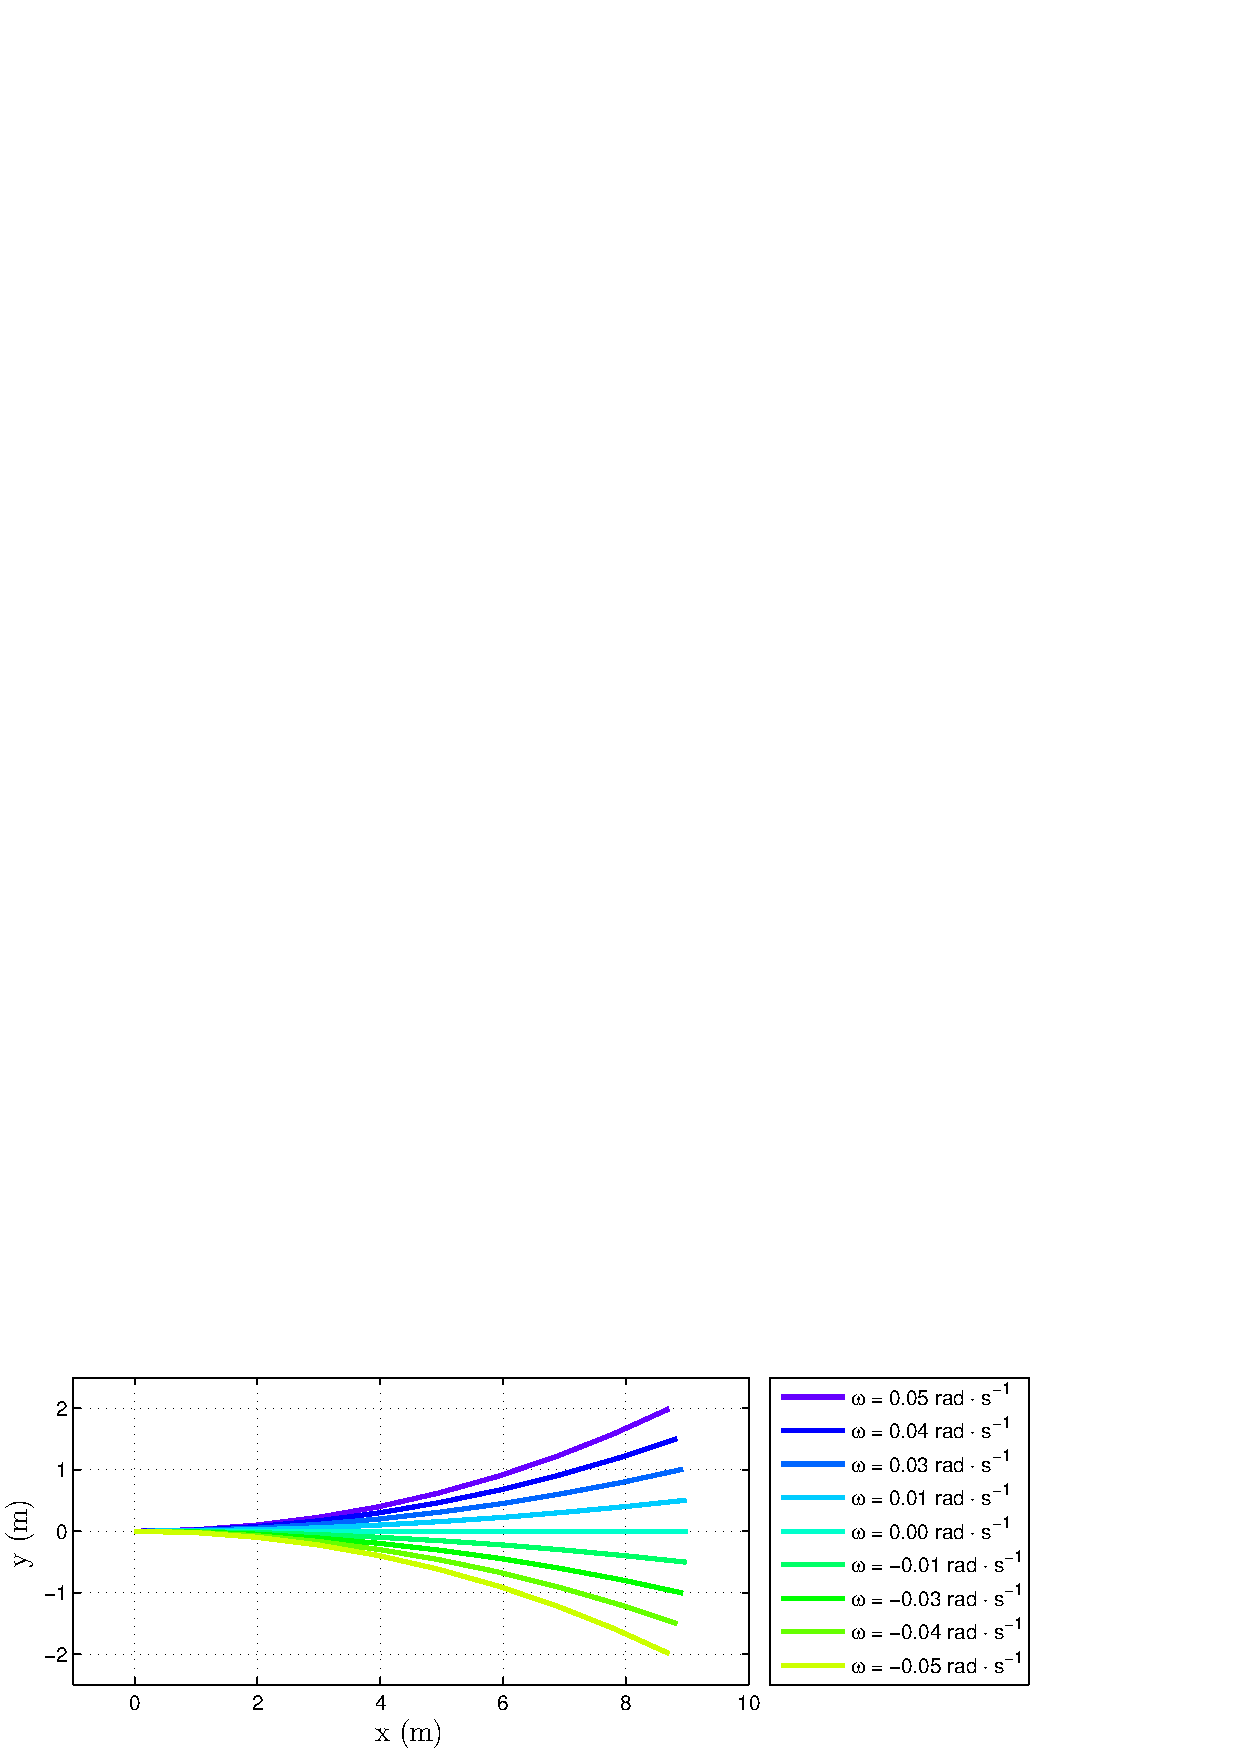
\includegraphics[width=0.9\textwidth]{motion_primitives.pdf}
  \caption{Nine motion primitives generated with $\omega = \{-0.05, -0.04,
  \dots, 0.05\}$ rad/s, $v = 1.0$ m/s.\label{fig:motion_prims}}
\end{figure}

Consider a robot following the arc of a
circle with velocity $v$ and rotational velocity $\omega$. Assuming the robot's
current position is given by $\mbf{x}_t=(x_t,y_t,\theta_t)^T$, forward-arc motion primitives
can be generated by specifying the future robot state, $\mbf{x}_{t+T}$,
as a function of $v$ and $\omega$ for a sequence of uniformly varying
times $T \in \mbb{R}^{+}$. These paths are described
by a set of nonlinear differential equations:
%
\eq{
  \dot{\mbf{x}}_{t+T}
  &=
  \bbm
  \dot{x} \\
  \dot{y} \\
  \dot{\theta}
  \ebm_{t+T}
  =
  \bbm
  v \cos
  \left(
  \theta_{t+T}
  \right) \\
  v \sin
  \left(
  \theta_{t+T}
  \right) \\
  \omega
  \ebm,
  \label{eq:arc_differential}
}
%
the solution of which is given by
%
\eq{
  \mbf{x}_{t+T}
  &=
  \bbm
  \frac{v}{\omega}
  \left(
  \sin
  \left(
  \omega T + \theta_{t}
  \right)
  -
  \sin
  \left(
  \theta_{t}
  \right)
  \right)
  \\
  \frac{v}{\omega}
  \left(
  \cos
  \left(
  \theta_{t}
  \right)
  -\cos
  \left(
  \omega T + \theta_{t}
  \right)
  \right)
  \\
  \omega T
  \ebm
  +
  \mbf{x}_{t}.
  \label{eq:motion_primitive_generator}
}
%
Sequentially incrementing $T$ in~\eqref{eq:motion_primitive_generator}
produces a sampling of poses lying along an arc
parameterized by the robot's velocity and angular velocity, with origin $\mbf{x}_{t}$.

A sampling of actions with varying $v$ and $w$ values (such as that depicted in
Fig.~\ref{fig:motion_prims}) is referred to as a
primitive \textit{dictionary}. To generate more actions, one can construct a
primitive \textit{library}. This is accomplished by forming a tree with nodes
corresponding to poses at the endpoints of actions. The tree is initialized by adding
the robot's current position as the root node. Then, a dictionary of motion
primitives is rotated and translated to leaf nodes in the tree until a specified
depth is reached. A primitive library is shown in
Fig.~\ref{fig:primitive_library}.
%
\begin{figure}
  \centering
  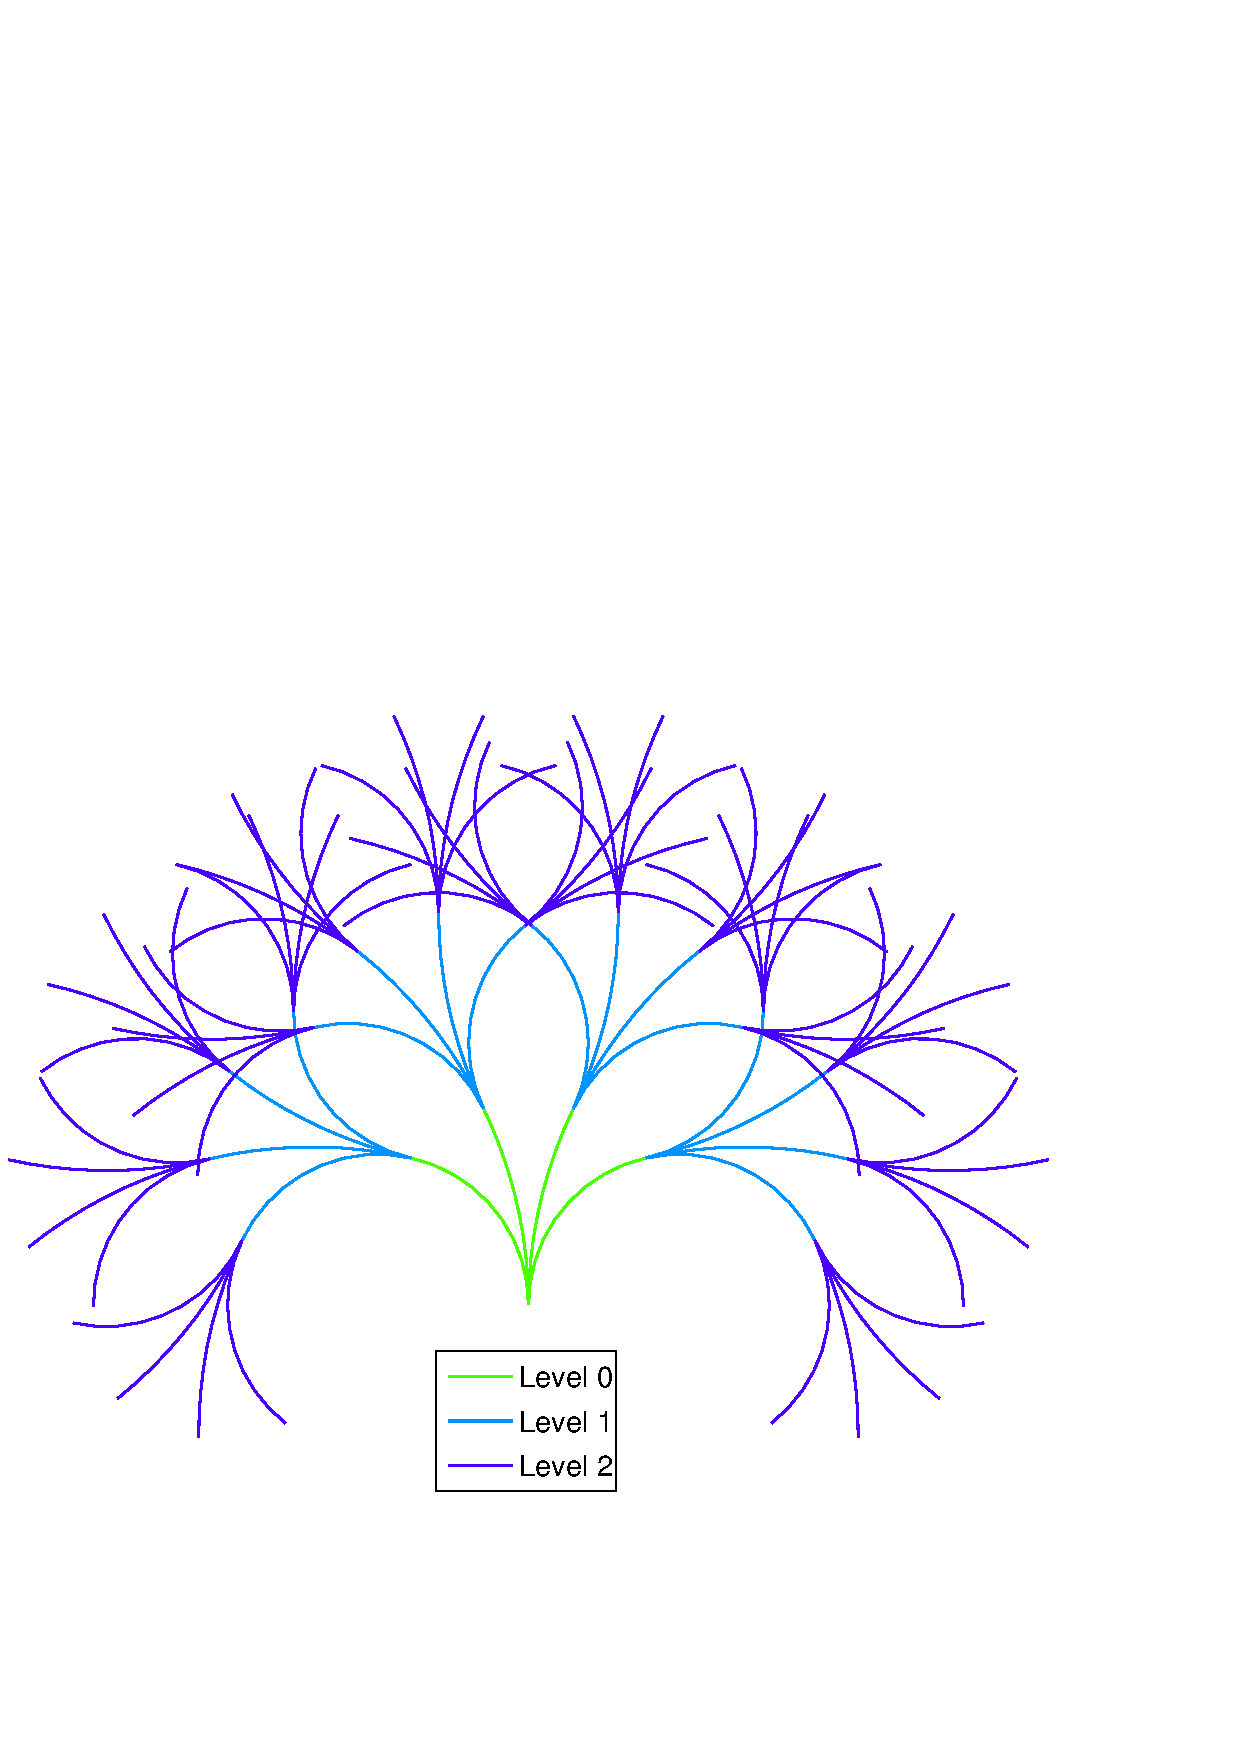
\includegraphics[width=0.7\textwidth, trim=10mm 45mm 10mm 80mm]{lattice_graph.pdf}
  \caption{A primitive dictionary with a depth of three constructed from a
  library of four motion primitives. \label{fig:primitive_library}}
\end{figure}

Forward-arc motion primitives are pre-computed prior to deployment into an
unknown environment, making them an efficient choice for real-time exploration. Collision
checking involves stepping along actions during a breadth-first or depth-first search and
pruning all nodes (actions) that lie below those that contain a collision.

\subsection{Lattice Graph Motion Primitives}
\label{subsec:lg_motion_primitives}

A third method for generating actions is lattice graph planning. Lattice graph
planners define a discrete set of goal states, and
solve Boundary Value Problems (BVPs) to find trajectories from $(\emptyset)$ to
each goal~\cite{pivtoraiko2005generating,pivtoraiko2009differentially,pivtoraiko2013incremental}
(Fig.~\ref{fig:lattice_graph}). The resulting set of motion primitives can
be rotated and translated to the robot's current position at run-time, and sampled
from to produce candidate actions. Like forward-arc motion primitives, lattice
graph motion primitives can be pre-computed and are therefore a suitable choice for
real-time exploration. Collision checking for motion primitives in the lattice
graph involves stepping along the action and checking for poses that lie outside
of the robot's configuration space.

\begin{figure}
  \centering
  \includegraphics[width=0.5\textwidth]{lattice_graph_white.png}
  \caption{An $11\times 11 \times 1$ lattice graph generated by solving a BVP
  from the robot's initial pose (middle, facing right) to a lattice of final
poses (with final angle equal to initial angle) subject to linear and angular velocity
constraints. No solution exists for the nodes immediately above and below the
robot's initial position. \label{fig:lattice_graph}}
\end{figure}

\section{Generalized Entropies and Divergences}
\label{sec:entropy_and_divergence}

Two fundamental building blocks of information theory are entropy and
divergence. The former describes the amount of uncertainty in a random variable,
or equivalently, the random variable's information content. The latter is a
distance metric between probability distributions that describes the
information lost when one distribution is used to describe another.
The most well-known forms of entropy and divergence are the Shannon
entropy~\cite{shannon1948mathematical}, and
Kullback-Leibler divergence~\cite{kullback1951information}. For a random variable
$X$, the Shannon entropy, $\text{H}$, and Kullback-Leibler divergence,
$\text{D}_{\text{KL}}$, are given by
%
\eq{
  \text{H}\left(X\right)
  &=
  - \sum_{x_{i} \in \mc{X}} P(x_{i}) \log_{2} P(x_{i}),
  \\
  \text{D}_{\text{KL}}
  \left(P \vert \vert Q\right)
  &=
  \sum_{x_{i} \in \mc{X}}
  P(x_{i})
  \log_{2}
  \frac
  {P(x_{i})}
  {Q(x_{i})},
}
%
where $\mc{X}$ is the sample space of $X$, and $P$ and $Q$ are discrete probability
distributions over $X$. While Shannon entropy and Kullback-Leibler divergence
succinctly describe critical concepts of information theory, alternative definitions of
these concepts exist.

Shannon entropy is one solution to a more general parametric family of
entropies introduced by R\'{e}nyi~\cite{renyi1961measures} that take the
(discrete) form
%
\eq{
  \text{H}_{\alpha}\left(X\right)
  &=
  \frac{1}{1-\alpha}
  \log_{2}
  \sum_{x_{i} \in \mc{X}}
  P^{\alpha}\left(x_{i}\right)
  \quad \text{(discrete)} \\
  \text{H}_{\alpha}\left(X\right)
  &=
  \frac{1}{1-\alpha}
  \log_{2}
  \int_{\mc{X}}
  p^{\alpha}\left(x\right)
  \quad \text{(continuous)}.
}
%
R\'{e}nyi's so-called \textit{$\alpha$-entropy} approaches the Shannon entropy as $\alpha
\rightarrow 1^{+}$, but allows one to express the information content of a
random variable using any choice from a family of functions. In some cases
$\text{H}_{\infty}$ entropy or $\text{H}_{2}$ entropy, for example, may be
easier to evaluate than Shannon entropy, and carry a similar meaning.
R\'{e}nyi's $\alpha$-entropy will be
used for an optimization that is difficult to solve using Shannon's entropy in
Chapter~\ref{chapter3}.

In a similar nature, there exists a spectrum of divergence measures that
generalize and extend the properties of the Kullback-Leibler divergence. The
Cauchy-Schwarz (CS) divergence is one measure that is of
particular importance to this thesis. CS divergence can be derived by
substituting two
distributions, $P$ and $Q$ into the Cauchy-Schwarz inequality~\cite{rudin1964principles}:
%
\eq{
  \sqrt{
    \sum_{x_{i} \in \mc{X}}
    P^{2}(x_{i})
    \sum_{x_{i} \in \mc{X}}
    Q^{2}(x_{i})
  }
  &\ge
  \sum_{x_{i} \in \mc{X}}
  P(x_{i})
  Q(x_{i})
  \quad \text{(discrete)} \\
  \sqrt{
    \int_{\mc{X}}
    p^{2}(x)dx
    \int_{\mc{X}}
    q^{2}(x)dx
  }
  &\ge
  \int_{\mc{X}}
  p(x)
  q(x)
  dx
  \quad \text{(continuous)}.
  \label{eq:cs_inequality}
}
%
CS divergence measures the extent of the inequality
in~\eqref{eq:cs_inequality}:
%
\eq{
  \text{D}_{\text{CS}}
  \left(P \vert \vert Q\right)
  &=
  \log
  \frac
  {
    \sum\limits_{x_{i} \in \mc{X}}
    P^{2}(x_{i})
    \sum\limits_{x_{i} \in \mc{X}}
    Q^{2}(x_{i})
  }
  {
    \left(
    \sum\limits_{x_{i} \in \mc{X}}
    P(x_{i})
    Q(x_{i})
    \right)^{2}
  }
  \quad \text{(discrete)}
  \\
  \text{D}_{\text{CS}}
  \left(p \vert \vert q\right)
  &=
  \log
  \frac
  {
    \int_{\mc{X}}
    p^{2}(x) dx
    \int_{\mc{X}}
    q^{2}(x) dx
  }
  {
    \left(
    \int_{\mc{X}}
    p(x)
    q(x)
    dx
    \right)^{2}
  }
  \quad \text{(continuous)}.
  \label{eq:cs_divergence}
}
%
CS divergence is a non-negative distance metric that takes on a value of zero
when its arguments are the same distribution. Unlike Kullback-Leibler
divergence, CS divergence is symmetric in its arguments. It can equivalently be written in
terms of R\'{e}nyi's $\alpha$-entropy for $\alpha=2$.
%
\eq
{
  \text{D}_{\text{CS}}
  \left(p(x) \vert \vert q(y)\right)
  &=
  -2\log
  \int_{\mc{X}, \mc{Y}}
  p(x) q(y)
  dx dy
  +
  \log
  \int_{\mc{X}}
  p^{2}(x)
  dx
  +
  \log
  \int_{\mc{Y}}
  q^{2}(y)
  dy \\
  &=
  2 \text{H}_{2}\left(X; Y\right)
  - \text{H}_{2}\left(X\right)
  - \text{H}_{2}\left(Y\right),
  \label{eq:csd_entropy_decomp}
}
%
where $\text{H}_{2}\left(X; Y\right)$ is the quadratic R\'{e}nyi
cross-entropy~\cite{rao2008learning}:
%
\eq
{
  \text{H}_{2}\left(X;Y\right)
  &=
  -\log_{2}
  \sum_{x_{i} \in \mc{X}, y_{i} \in \mc{Y}}
  P(x_{i})Q(y_{i})
  \quad \text{(discrete)}
  \\
  \text{H}_{2}\left(X;Y\right)
  &=
  -\log_{2}
  \int
  p(x)
  q(y)
  dx dy
  \quad \text{(continuous)}.
}

\section{Cauchy-Schwarz Quadratic Mutual Information}
\label{sec:csqmi}

The CS divergence metric described in Section~\ref{sec:entropy_and_divergence} can be
used to define a second distance metric that measures the amount of dependence
between two random variables $X$ and $Y$. The amount of dependence between two
random variables is synonymous with the definition of mutual information, another
fundamental building block of information theory. Mutual information metrics
describe the difference between a joint distribution, $p(x, y)$, and the product
of its marginals, $p(x)p(y)$. Like entropy and divergence, there exists a common
definition for mutual information (the \textit{Shannon mutual information} (SMI)) that can be
extended and generalized. In the context of mobile robotic exploration, a more convenient
definition of mutual information is the \textit{Cauchy-Schwarz Quadratic mutual
information} (CSQMI), which is derived
by substituting $p(x, y)$ for $p$ and $p(x)p(y)$ for $q$
in~\eqref{eq:cs_divergence}.
%
\eq{
  \text{I}_{\text{CS}}
  \left(
    X;
    Y
  \right)
  &=
  \log
  \frac
  {
    \int_{\mc{X}}
    \int_{\mc{Y}}
    p^{2}(x,y) dx dy
    \int_{\mc{X}}
    \int_{\mc{Y}}
    p^{2}(x)p^{2}(y) dx dy
  }
  {
    \left(
    \int_{\mc{X}}
    \int_{\mc{Y}}
    p(x,y)
    p(x)p(y)
    dx dy
    \right)^{2}
  }.
}
%
Charrow et al. originally showed that the CSQMI between a robot's map and a beam-based
sensor measurement is a superior reward metric to SMI for
exploration~\cite{charrow2015icra}. This is because CSQMI can be computed
analytically without requiring an expensive sampling step to
calculate the expected value of a future sensor measurement. Additionally,
CSQMI can be computed exactly in $\mc{O}(n^2)$, and to a close approximation
in $\mc{O}(n)$, where $n$ is the number of cells in the robot's map intersected by a
sequence of beam-based sensor measurements $z_{\tau}$. While SMI can also be approximated in time linear in
$n$, Charrow et al. show that CSQMI has a smaller linear constant factor,
allowing CSQMI to be computed in roughly one seventh of the amount of time.
Like SMI, CSQMI is non-negative and zero only when its arguments are independent
(i.e. when $p(x, y) = p(x)p(y)$). Figure~\ref{fig:mi_vs_csqmi} shows that CSQMI and SMI are
similar when evaluated on an OG with a beam-based sensor model, and control actions
that maximize CSQMI guide the robot to unexplored space. For discussion regarding
explicit calculation of CSQMI, the reader should refer to Charrow et al.~\cite{charrow2015icra}.

$\text{I}_{\text{CS}}\left(\mbf{m};\mbf{z}_{\mbf{\tau}}\left(\mbf{x}_{\mbf{\tau}}\right)\right)$
is therefore a suitable choice
for $\mc{J}\left(\mbf{m}; \mbf{z}_{\mbf{\tau}}\left(\mbf{x}_{\mbf{\tau}}\right)\right)$
in~\eqref{eq:active_perception}. The map $\mbf{m}$ is
considered to be a discrete multivariate random variable because its sample space is
discrete (cells may only be $\texttt{OCC}$ or $\texttt{EMP}$), so CSQMI between
an OG map and sequence of beam-based measurements is
%
\eq{
  \text{I}_{\text{CS}}
  \left(
  \mbf{m}; \mbf{z}_{\mbf{\tau}}
  \right)
  &=
  \log
  \frac
  {
    \int
    \sum_{\mc{M}}
    p^{2}(\mbf{m}, \mbf{z}_{\mbf{\tau}})
    d\mbf{z}_{\mbf{\tau}}
    \int
    \sum_{M}
    p^{2}(\mbf{m}) p^{2}(\mbf{z}_{\mbf{\tau}})
    d\mbf{z}_{\mbf{\tau}}
  }
  {
    \left(
    \int
    \sum_{\mc{M}}
    p(\mbf{m})p(\mbf{z}_{\mbf{\tau}})
    p(\mbf{m}, \mbf{z}_{\mbf{\tau}})
    d\mbf{z}_{\mbf{\tau}}
    \right)^{2}
  },
}
%
where $\mc{M}$ is a set of all possible map permutations. Substituting
$\text{I}_{\text{CS}}$ for $\mc{J}$ in~\eqref{eq:active_perception} yields
an active perception optimization that guides a robot towards unexplored
locations in its map by maximizing an information-theoretic reward functional.
%
\eq
{
 \mbf{x}_{\mbf{\tau}}^{*}
 &=
 \argmax_{\mbf{x}_{\mbf{\tau}} \in \mc{X}}
 \
 \text{I}_{\text{CS}}\left(\mbf{m},
 \mbf{z}_{\mbf{\tau}}(\mbf{x}_{\mbf{\tau}})\right).
 \label{eq:active_perception_csqmi}
}

\section{Summary of Foundations}

Chapter~\ref{chapter2} reviewed foundational elements that will be used for
derivations in the remaining chapters. These elements culminate in an
optimization that drives a robot towards unexplored space in its map by
maximizing an information-theoretic reward
function~\eqref{eq:active_perception_csqmi}. The chosen reward function,
CSQMI~\cite{principe2010information},
resembles Shannon's original definition of mutual information, but can be computed
more efficiently when its arguments are an OG map and a sequence
time-ordered beam-based sensor measurements~\cite{charrow2015icra}.

Furthermore, Chapter~\ref{chapter2} discussed three methods for generating
dynamically feasible and collision-free actions through the robot's
configuration space. The action maximizing CSQMI (either integrated over the
path, or at the action's final pose) will be chosen as that which optimally
drives the robot towards unexplored space. The remainder of this thesis will use both forward-arc
motion primitives and lattice graph motion primitives for action generation,
although the third option - frontier seeding - is equally viable.
